\documentclass{standalone}
\usepackage{tikz}
\usetikzlibrary{patterns, positioning}

\begin{document}
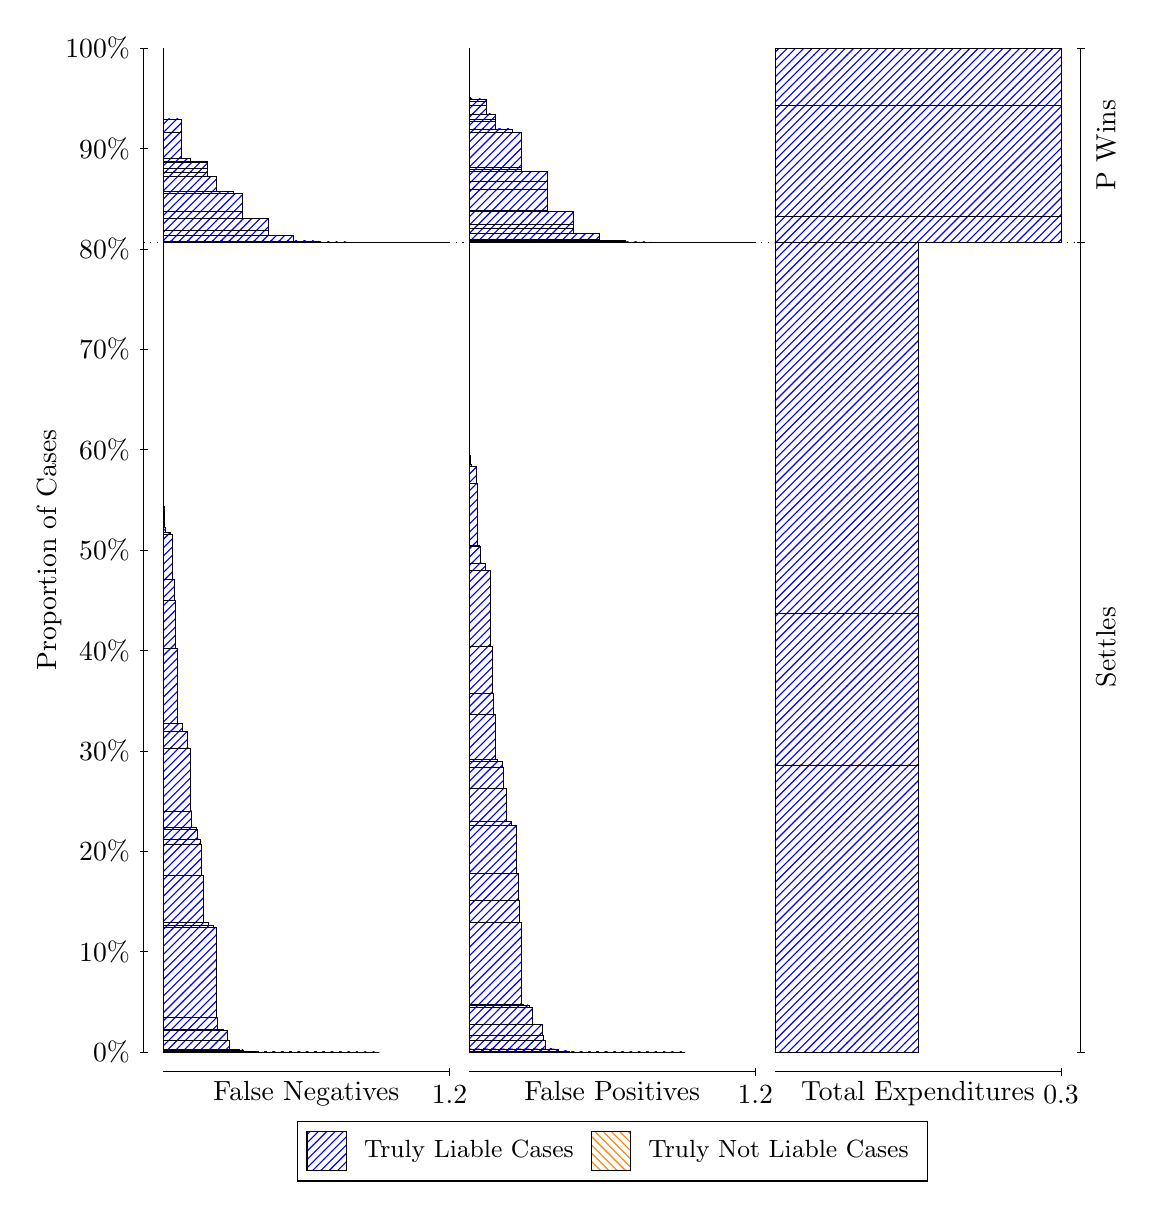
\begin{tikzpicture}
\draw[black, very thin] (1.5,1.75) -- (1.5,14.5);
\node[rotate=90, anchor=center] at (0.3, 8.125) {Proportion of Cases};
\draw[black, very thin] (1.45,1.75) -- (1.55,1.75);
\node[anchor=east] at (1.45, 1.75) {0\%};
\draw[black, very thin] (1.45,3.025) -- (1.55,3.025);
\node[anchor=east] at (1.45, 3.025) {10\%};
\draw[black, very thin] (1.45,4.3) -- (1.55,4.3);
\node[anchor=east] at (1.45, 4.3) {20\%};
\draw[black, very thin] (1.45,5.575) -- (1.55,5.575);
\node[anchor=east] at (1.45, 5.575) {30\%};
\draw[black, very thin] (1.45,6.85) -- (1.55,6.85);
\node[anchor=east] at (1.45, 6.85) {40\%};
\draw[black, very thin] (1.45,8.125) -- (1.55,8.125);
\node[anchor=east] at (1.45, 8.125) {50\%};
\draw[black, very thin] (1.45,9.4) -- (1.55,9.4);
\node[anchor=east] at (1.45, 9.4) {60\%};
\draw[black, very thin] (1.45,10.675) -- (1.55,10.675);
\node[anchor=east] at (1.45, 10.675) {70\%};
\draw[black, very thin] (1.45,11.95) -- (1.55,11.95);
\node[anchor=east] at (1.45, 11.95) {80\%};
\draw[black, very thin] (1.45,13.225) -- (1.55,13.225);
\node[anchor=east] at (1.45, 13.225) {90\%};
\draw[black, very thin] (1.45,14.5) -- (1.55,14.5);
\node[anchor=east] at (1.45, 14.5) {100\%};

\draw[black, very thin] (13.4,1.75) -- (13.4,14.5);
\draw[black, very thin] (13.35,1.75) -- (13.45,1.75);
\node[anchor=west] at (13.35, 1.75) {};
\draw[black, very thin] (13.35,12.035) -- (13.45,12.035);
\node[anchor=west] at (13.35, 12.035) {};
\draw[black, very thin] (13.35,14.5) -- (13.45,14.5);
\node[anchor=west] at (13.35, 14.5) {};

\draw[black, very thin, pattern color=blue, pattern=north east lines] (1.75,1.75) rectangle (4.4935,1.75);
\draw[black, very thin, pattern color=blue, pattern=north east lines] (1.75,1.75) rectangle (4.1969,1.75);
\draw[black, very thin, pattern color=blue, pattern=north east lines] (1.75,1.75) rectangle (4.164,1.75);
\draw[black, very thin, pattern color=blue, pattern=north east lines] (1.75,1.75) rectangle (4.0486,1.75);
\draw[black, very thin, pattern color=blue, pattern=north east lines] (1.75,1.75) rectangle (3.9003,1.75);
\draw[black, very thin, pattern color=blue, pattern=north east lines] (1.75,1.75) rectangle (3.8674,1.75);
\draw[black, very thin, pattern color=blue, pattern=north east lines] (1.75,1.75) rectangle (3.8344,1.75);
\draw[black, very thin, pattern color=blue, pattern=north east lines] (1.75,1.75) rectangle (3.752,1.75);
\draw[black, very thin, pattern color=blue, pattern=north east lines] (1.75,1.75) rectangle (3.7191,1.75);
\draw[black, very thin, pattern color=blue, pattern=north east lines] (1.75,1.75) rectangle (3.6037,1.75);
\draw[black, very thin, pattern color=blue, pattern=north east lines] (1.75,1.75) rectangle (3.5708,1.75);
\draw[black, very thin, pattern color=blue, pattern=north east lines] (1.75,1.75) rectangle (3.5378,1.75);
\draw[black, very thin, pattern color=blue, pattern=north east lines] (1.75,1.75) rectangle (3.5049,1.75);
\draw[black, very thin, pattern color=blue, pattern=north east lines] (1.75,1.75) rectangle (3.4554,1.75);
\draw[black, very thin, pattern color=blue, pattern=north east lines] (1.75,1.75) rectangle (3.4225,1.75);
\draw[black, very thin, pattern color=blue, pattern=north east lines] (1.75,1.75) rectangle (3.3895,1.75);
\draw[black, very thin, pattern color=blue, pattern=north east lines] (1.75,1.75) rectangle (3.3071,1.75);
\draw[black, very thin, pattern color=blue, pattern=north east lines] (1.75,1.75) rectangle (3.2742,1.75);
\draw[black, very thin, pattern color=blue, pattern=north east lines] (1.75,1.75) rectangle (3.2412,1.7501);
\draw[black, very thin, pattern color=blue, pattern=north east lines] (1.75,1.7501) rectangle (3.2083,1.7501);
\draw[black, very thin, pattern color=blue, pattern=north east lines] (1.75,1.7501) rectangle (3.1753,1.7501);
\draw[black, very thin, pattern color=blue, pattern=north east lines] (1.75,1.7501) rectangle (3.1588,1.7501);
\draw[black, very thin, pattern color=blue, pattern=north east lines] (1.75,1.7501) rectangle (3.1259,1.7501);
\draw[black, very thin, pattern color=blue, pattern=north east lines] (1.75,1.7501) rectangle (3.0929,1.7505);
\draw[black, very thin, pattern color=blue, pattern=north east lines] (1.75,1.7505) rectangle (3.06,1.7505);
\draw[black, very thin, pattern color=blue, pattern=north east lines] (1.75,1.7505) rectangle (2.9776,1.7506);
\draw[black, very thin, pattern color=blue, pattern=north east lines] (1.75,1.7506) rectangle (2.9446,1.7506);
\draw[black, very thin, pattern color=blue, pattern=north east lines] (1.75,1.7506) rectangle (2.9117,1.7563);
\draw[black, very thin, pattern color=blue, pattern=north east lines] (1.75,1.7563) rectangle (2.8787,1.7563);
\draw[black, very thin, pattern color=blue, pattern=north east lines] (1.75,1.7563) rectangle (2.8458,1.7564);
\draw[black, very thin, pattern color=blue, pattern=north east lines] (1.75,1.7564) rectangle (2.8293,1.7567);
\draw[black, very thin, pattern color=blue, pattern=north east lines] (1.75,1.7567) rectangle (2.7963,1.7567);
\draw[black, very thin, pattern color=blue, pattern=north east lines] (1.75,1.7567) rectangle (2.7634,1.7773);
\draw[black, very thin, pattern color=blue, pattern=north east lines] (1.75,1.7773) rectangle (2.7304,1.7774);
\draw[black, very thin, pattern color=blue, pattern=north east lines] (1.75,1.7774) rectangle (2.7139,1.7785);
\draw[black, very thin, pattern color=blue, pattern=north east lines] (1.75,1.7785) rectangle (2.648,1.7804);
\draw[black, very thin, pattern color=blue, pattern=north east lines] (1.75,1.7804) rectangle (2.6151,1.7804);
\draw[black, very thin, pattern color=blue, pattern=north east lines] (1.75,1.7804) rectangle (2.5821,1.9016);
\draw[black, very thin, pattern color=blue, pattern=north east lines] (1.75,1.9016) rectangle (2.5656,2.0237);
\draw[black, very thin, pattern color=blue, pattern=north east lines] (1.75,2.0237) rectangle (2.5492,2.0291);
\draw[black, very thin, pattern color=blue, pattern=north east lines] (1.75,2.0291) rectangle (2.5162,2.0348);
\draw[black, very thin, pattern color=blue, pattern=north east lines] (1.75,2.0348) rectangle (2.4997,2.0402);
\draw[black, very thin, pattern color=blue, pattern=north east lines] (1.75,2.0402) rectangle (2.4668,2.0403);
\draw[black, very thin, pattern color=blue, pattern=north east lines] (1.75,2.0403) rectangle (2.4338,2.1908);
\draw[black, very thin, pattern color=blue, pattern=north east lines] (1.75,2.1908) rectangle (2.4173,3.3323);
\draw[black, very thin, pattern color=blue, pattern=north east lines] (1.75,3.3323) rectangle (2.4009,3.3342);
\draw[black, very thin, pattern color=blue, pattern=north east lines] (1.75,3.3342) rectangle (2.3844,3.3615);
\draw[black, very thin, pattern color=blue, pattern=north east lines] (1.75,3.3615) rectangle (2.3185,3.3942);
\draw[black, very thin, pattern color=blue, pattern=north east lines] (1.75,3.3942) rectangle (2.2855,3.3942);
\draw[black, very thin, pattern color=blue, pattern=north east lines] (1.75,3.3942) rectangle (2.2526,3.9929);
\draw[black, very thin, pattern color=blue, pattern=north east lines] (1.75,3.9929) rectangle (2.2361,4.384);
\draw[black, very thin, pattern color=blue, pattern=north east lines] (1.75,4.384) rectangle (2.2196,4.4576);
\draw[black, very thin, pattern color=blue, pattern=north east lines] (1.75,4.4576) rectangle (2.1867,4.5756);
\draw[black, very thin, pattern color=blue, pattern=north east lines] (1.75,4.5756) rectangle (2.1702,4.6019);
\draw[black, very thin, pattern color=blue, pattern=north east lines] (1.75,4.6019) rectangle (2.1372,4.6019);
\draw[black, very thin, pattern color=blue, pattern=north east lines] (1.75,4.6019) rectangle (2.1043,4.8131);
\draw[black, very thin, pattern color=blue, pattern=north east lines] (1.75,4.8131) rectangle (2.0878,5.6055);
\draw[black, very thin, pattern color=blue, pattern=north east lines] (1.75,5.6055) rectangle (2.0713,5.6106);
\draw[black, very thin, pattern color=blue, pattern=north east lines] (1.75,5.6106) rectangle (2.0548,5.8244);
\draw[black, very thin, pattern color=blue, pattern=north east lines] (1.75,5.8244) rectangle (1.9889,5.9195);
\draw[black, very thin, pattern color=blue, pattern=north east lines] (1.75,5.9195) rectangle (1.956,5.9199);
\draw[black, very thin, pattern color=blue, pattern=north east lines] (1.75,5.9199) rectangle (1.923,6.8774);
\draw[black, very thin, pattern color=blue, pattern=north east lines] (1.75,6.8774) rectangle (1.9065,7.4837);
\draw[black, very thin, pattern color=blue, pattern=north east lines] (1.75,7.4837) rectangle (1.8901,7.7511);
\draw[black, very thin, pattern color=blue, pattern=north east lines] (1.75,7.7511) rectangle (1.8571,8.3224);
\draw[black, very thin, pattern color=blue, pattern=north east lines] (1.75,8.3224) rectangle (1.8406,8.3486);
\draw[black, very thin, pattern color=blue, pattern=north east lines] (1.75,8.3486) rectangle (1.8077,8.3487);
\draw[black, very thin, pattern color=blue, pattern=north east lines] (1.75,8.3487) rectangle (1.7747,8.4157);
\draw[black, very thin, pattern color=blue, pattern=north east lines] (1.75,8.4157) rectangle (1.7582,8.6831);
\draw[black, very thin, pattern color=orange, pattern=north west lines] (1.75,8.6831) rectangle (1.75,8.6831);
\draw[black, very thin, pattern color=blue, pattern=north east lines] (1.75,8.6831) rectangle (1.75,12.035);
\draw[black, very thin, pattern color=blue, pattern=north east lines] (1.75,12.035) rectangle (5.3833,12.035);
\draw[black, very thin, pattern color=blue, pattern=north east lines] (1.75,12.035) rectangle (5.0538,12.035);
\draw[black, very thin, pattern color=blue, pattern=north east lines] (1.75,12.035) rectangle (4.7242,12.035);
\draw[black, very thin, pattern color=blue, pattern=north east lines] (1.75,12.035) rectangle (4.3947,12.035);
\draw[black, very thin, pattern color=blue, pattern=north east lines] (1.75,12.035) rectangle (4.2793,12.035);
\draw[black, very thin, pattern color=blue, pattern=north east lines] (1.75,12.035) rectangle (4.0651,12.036);
\draw[black, very thin, pattern color=blue, pattern=north east lines] (1.75,12.036) rectangle (4.0651,12.037);
\draw[black, very thin, pattern color=blue, pattern=north east lines] (1.75,12.037) rectangle (3.9498,12.037);
\draw[black, very thin, pattern color=blue, pattern=north east lines] (1.75,12.037) rectangle (3.7356,12.044);
\draw[black, very thin, pattern color=blue, pattern=north east lines] (1.75,12.044) rectangle (3.7356,12.051);
\draw[black, very thin, pattern color=blue, pattern=north east lines] (1.75,12.051) rectangle (3.6202,12.051);
\draw[black, very thin, pattern color=blue, pattern=north east lines] (1.75,12.051) rectangle (3.406,12.117);
\draw[black, very thin, pattern color=blue, pattern=north east lines] (1.75,12.117) rectangle (3.406,12.12);
\draw[black, very thin, pattern color=blue, pattern=north east lines] (1.75,12.12) rectangle (3.2907,12.12);
\draw[black, very thin, pattern color=blue, pattern=north east lines] (1.75,12.12) rectangle (3.2907,12.12);
\draw[black, very thin, pattern color=blue, pattern=north east lines] (1.75,12.12) rectangle (3.0765,12.188);
\draw[black, very thin, pattern color=blue, pattern=north east lines] (1.75,12.188) rectangle (3.0765,12.332);
\draw[black, very thin, pattern color=blue, pattern=north east lines] (1.75,12.332) rectangle (2.9611,12.332);
\draw[black, very thin, pattern color=blue, pattern=north east lines] (1.75,12.332) rectangle (2.9611,12.332);
\draw[black, very thin, pattern color=blue, pattern=north east lines] (1.75,12.332) rectangle (2.9611,12.333);
\draw[black, very thin, pattern color=blue, pattern=north east lines] (1.75,12.333) rectangle (2.7469,12.425);
\draw[black, very thin, pattern color=blue, pattern=north east lines] (1.75,12.425) rectangle (2.7469,12.651);
\draw[black, very thin, pattern color=blue, pattern=north east lines] (1.75,12.651) rectangle (2.7469,12.658);
\draw[black, very thin, pattern color=blue, pattern=north east lines] (1.75,12.658) rectangle (2.6316,12.658);
\draw[black, very thin, pattern color=blue, pattern=north east lines] (1.75,12.658) rectangle (2.6316,12.677);
\draw[black, very thin, pattern color=blue, pattern=north east lines] (1.75,12.677) rectangle (2.6316,12.68);
\draw[black, very thin, pattern color=blue, pattern=north east lines] (1.75,12.68) rectangle (2.4173,12.87);
\draw[black, very thin, pattern color=blue, pattern=north east lines] (1.75,12.87) rectangle (2.302,12.928);
\draw[black, very thin, pattern color=blue, pattern=north east lines] (1.75,12.928) rectangle (2.302,12.969);
\draw[black, very thin, pattern color=blue, pattern=north east lines] (1.75,12.969) rectangle (2.302,13.047);
\draw[black, very thin, pattern color=blue, pattern=north east lines] (1.75,13.047) rectangle (2.302,13.063);
\draw[black, very thin, pattern color=blue, pattern=north east lines] (1.75,13.063) rectangle (2.0878,13.063);
\draw[black, very thin, pattern color=blue, pattern=north east lines] (1.75,13.063) rectangle (2.0878,13.103);
\draw[black, very thin, pattern color=blue, pattern=north east lines] (1.75,13.103) rectangle (2.0878,13.103);
\draw[black, very thin, pattern color=blue, pattern=north east lines] (1.75,13.103) rectangle (1.9724,13.43);
\draw[black, very thin, pattern color=blue, pattern=north east lines] (1.75,13.43) rectangle (1.9724,13.6);
\draw[black, very thin, pattern color=blue, pattern=north east lines] (1.75,13.6) rectangle (1.7582,13.6);
\draw[black, very thin, pattern color=blue, pattern=north east lines] (1.75,13.6) rectangle (1.7582,13.6);
\draw[black, very thin, pattern color=orange, pattern=north west lines] (1.75,13.6) rectangle (1.75,13.6);
\draw[black, very thin, pattern color=blue, pattern=north east lines] (1.75,13.6) rectangle (1.75,14.5);
\draw[black, very thin, pattern color=orange, pattern=north west lines] (5.6333,1.75) rectangle (8.3769,1.75);
\draw[black, very thin, pattern color=blue, pattern=north east lines] (5.6333,1.75) rectangle (8.3769,1.75);
\draw[black, very thin, pattern color=orange, pattern=north west lines] (5.6333,1.75) rectangle (8.2286,1.75);
\draw[black, very thin, pattern color=blue, pattern=north east lines] (5.6333,1.75) rectangle (8.2286,1.75);
\draw[black, very thin, pattern color=orange, pattern=north west lines] (5.6333,1.75) rectangle (8.0803,1.75);
\draw[black, very thin, pattern color=blue, pattern=north east lines] (5.6333,1.75) rectangle (8.0803,1.75);
\draw[black, very thin, pattern color=blue, pattern=north east lines] (5.6333,1.75) rectangle (8.0473,1.75);
\draw[black, very thin, pattern color=blue, pattern=north east lines] (5.6333,1.75) rectangle (7.899,1.75);
\draw[black, very thin, pattern color=blue, pattern=north east lines] (5.6333,1.75) rectangle (7.7507,1.75);
\draw[black, very thin, pattern color=blue, pattern=north east lines] (5.6333,1.75) rectangle (7.7178,1.75);
\draw[black, very thin, pattern color=orange, pattern=north west lines] (5.6333,1.75) rectangle (7.6354,1.75);
\draw[black, very thin, pattern color=blue, pattern=north east lines] (5.6333,1.75) rectangle (7.6354,1.75);
\draw[black, very thin, pattern color=blue, pattern=north east lines] (5.6333,1.75) rectangle (7.5695,1.75);
\draw[black, very thin, pattern color=orange, pattern=north west lines] (5.6333,1.75) rectangle (7.4871,1.75);
\draw[black, very thin, pattern color=blue, pattern=north east lines] (5.6333,1.75) rectangle (7.4871,1.75);
\draw[black, very thin, pattern color=blue, pattern=north east lines] (5.6333,1.75) rectangle (7.4212,1.75);
\draw[black, very thin, pattern color=blue, pattern=north east lines] (5.6333,1.75) rectangle (7.3882,1.75);
\draw[black, very thin, pattern color=orange, pattern=north west lines] (5.6333,1.75) rectangle (7.3388,1.75);
\draw[black, very thin, pattern color=blue, pattern=north east lines] (5.6333,1.75) rectangle (7.3388,1.75);
\draw[black, very thin, pattern color=blue, pattern=north east lines] (5.6333,1.75) rectangle (7.3058,1.75);
\draw[black, very thin, pattern color=blue, pattern=north east lines] (5.6333,1.75) rectangle (7.2399,1.75);
\draw[black, very thin, pattern color=orange, pattern=north west lines] (5.6333,1.75) rectangle (7.1905,1.75);
\draw[black, very thin, pattern color=blue, pattern=north east lines] (5.6333,1.75) rectangle (7.1905,1.75);
\draw[black, very thin, pattern color=blue, pattern=north east lines] (5.6333,1.75) rectangle (7.1575,1.75);
\draw[black, very thin, pattern color=blue, pattern=north east lines] (5.6333,1.75) rectangle (7.0916,1.7505);
\draw[black, very thin, pattern color=blue, pattern=north east lines] (5.6333,1.7505) rectangle (7.0587,1.7505);
\draw[black, very thin, pattern color=orange, pattern=north west lines] (5.6333,1.7505) rectangle (7.0422,1.7505);
\draw[black, very thin, pattern color=blue, pattern=north east lines] (5.6333,1.7505) rectangle (7.0422,1.7505);
\draw[black, very thin, pattern color=blue, pattern=north east lines] (5.6333,1.7505) rectangle (7.0092,1.7505);
\draw[black, very thin, pattern color=blue, pattern=north east lines] (5.6333,1.7505) rectangle (6.9763,1.7505);
\draw[black, very thin, pattern color=blue, pattern=north east lines] (5.6333,1.7505) rectangle (6.9104,1.753);
\draw[black, very thin, pattern color=orange, pattern=north west lines] (5.6333,1.753) rectangle (6.8939,1.753);
\draw[black, very thin, pattern color=blue, pattern=north east lines] (5.6333,1.753) rectangle (6.8939,1.7649);
\draw[black, very thin, pattern color=blue, pattern=north east lines] (5.6333,1.7649) rectangle (6.8609,1.7649);
\draw[black, very thin, pattern color=blue, pattern=north east lines] (5.6333,1.7649) rectangle (6.828,1.7651);
\draw[black, very thin, pattern color=blue, pattern=north east lines] (5.6333,1.7651) rectangle (6.7621,1.7889);
\draw[black, very thin, pattern color=orange, pattern=north west lines] (5.6333,1.7889) rectangle (6.7456,1.7889);
\draw[black, very thin, pattern color=blue, pattern=north east lines] (5.6333,1.7889) rectangle (6.7456,1.7889);
\draw[black, very thin, pattern color=blue, pattern=north east lines] (5.6333,1.7889) rectangle (6.7291,1.7894);
\draw[black, very thin, pattern color=blue, pattern=north east lines] (5.6333,1.7894) rectangle (6.7126,1.7895);
\draw[black, very thin, pattern color=blue, pattern=north east lines] (5.6333,1.7895) rectangle (6.6797,1.7895);
\draw[black, very thin, pattern color=blue, pattern=north east lines] (5.6333,1.7895) rectangle (6.6467,1.7898);
\draw[black, very thin, pattern color=orange, pattern=north west lines] (5.6333,1.7898) rectangle (6.5973,1.7898);
\draw[black, very thin, pattern color=blue, pattern=north east lines] (5.6333,1.7898) rectangle (6.5973,1.9011);
\draw[black, very thin, pattern color=blue, pattern=north east lines] (5.6333,1.9011) rectangle (6.5808,1.9594);
\draw[black, very thin, pattern color=blue, pattern=north east lines] (5.6333,1.9594) rectangle (6.5643,2.0986);
\draw[black, very thin, pattern color=blue, pattern=north east lines] (5.6333,2.0986) rectangle (6.5314,2.0987);
\draw[black, very thin, pattern color=blue, pattern=north east lines] (5.6333,2.0987) rectangle (6.4984,2.1053);
\draw[black, very thin, pattern color=blue, pattern=north east lines] (5.6333,2.1053) rectangle (6.4325,2.3165);
\draw[black, very thin, pattern color=blue, pattern=north east lines] (5.6333,2.3165) rectangle (6.416,2.3167);
\draw[black, very thin, pattern color=blue, pattern=north east lines] (5.6333,2.3167) rectangle (6.3995,2.3429);
\draw[black, very thin, pattern color=blue, pattern=north east lines] (5.6333,2.3429) rectangle (6.3831,2.3482);
\draw[black, very thin, pattern color=blue, pattern=north east lines] (5.6333,2.3482) rectangle (6.3501,2.3482);
\draw[black, very thin, pattern color=blue, pattern=north east lines] (5.6333,2.3482) rectangle (6.3172,2.3536);
\draw[black, very thin, pattern color=orange, pattern=north west lines] (5.6333,2.3536) rectangle (6.3007,2.3536);
\draw[black, very thin, pattern color=blue, pattern=north east lines] (5.6333,2.3536) rectangle (6.3007,3.3942);
\draw[black, very thin, pattern color=blue, pattern=north east lines] (5.6333,3.3942) rectangle (6.2677,3.6761);
\draw[black, very thin, pattern color=blue, pattern=north east lines] (5.6333,3.6761) rectangle (6.2512,4.0168);
\draw[black, very thin, pattern color=blue, pattern=north east lines] (5.6333,4.0168) rectangle (6.2348,4.6231);
\draw[black, very thin, pattern color=blue, pattern=north east lines] (5.6333,4.6231) rectangle (6.2018,4.6236);
\draw[black, very thin, pattern color=blue, pattern=north east lines] (5.6333,4.6236) rectangle (6.1689,4.6765);
\draw[black, very thin, pattern color=blue, pattern=north east lines] (5.6333,4.6765) rectangle (6.1029,5.0997);
\draw[black, very thin, pattern color=blue, pattern=north east lines] (5.6333,5.0997) rectangle (6.0865,5.102);
\draw[black, very thin, pattern color=blue, pattern=north east lines] (5.6333,5.102) rectangle (6.07,5.3695);
\draw[black, very thin, pattern color=blue, pattern=north east lines] (5.6333,5.3695) rectangle (6.0535,5.4365);
\draw[black, very thin, pattern color=blue, pattern=north east lines] (5.6333,5.4365) rectangle (6.0206,5.4365);
\draw[black, very thin, pattern color=blue, pattern=north east lines] (5.6333,5.4365) rectangle (5.9876,5.4628);
\draw[black, very thin, pattern color=blue, pattern=north east lines] (5.6333,5.4628) rectangle (5.9711,6.034);
\draw[black, very thin, pattern color=blue, pattern=north east lines] (5.6333,6.034) rectangle (5.9382,6.3015);
\draw[black, very thin, pattern color=blue, pattern=north east lines] (5.6333,6.3015) rectangle (5.9217,6.9077);
\draw[black, very thin, pattern color=blue, pattern=north east lines] (5.6333,6.9077) rectangle (5.9052,7.8652);
\draw[black, very thin, pattern color=blue, pattern=north east lines] (5.6333,7.8652) rectangle (5.8723,7.8657);
\draw[black, very thin, pattern color=blue, pattern=north east lines] (5.6333,7.8657) rectangle (5.8393,7.9607);
\draw[black, very thin, pattern color=blue, pattern=north east lines] (5.6333,7.9607) rectangle (5.7734,8.1746);
\draw[black, very thin, pattern color=blue, pattern=north east lines] (5.6333,8.1746) rectangle (5.7569,8.1797);
\draw[black, very thin, pattern color=blue, pattern=north east lines] (5.6333,8.1797) rectangle (5.7404,8.9721);
\draw[black, very thin, pattern color=blue, pattern=north east lines] (5.6333,8.9721) rectangle (5.724,9.1833);
\draw[black, very thin, pattern color=blue, pattern=north east lines] (5.6333,9.1833) rectangle (5.691,9.1833);
\draw[black, very thin, pattern color=blue, pattern=north east lines] (5.6333,9.1833) rectangle (5.658,9.2096);
\draw[black, very thin, pattern color=blue, pattern=north east lines] (5.6333,9.2096) rectangle (5.6416,9.3276);
\draw[black, very thin, pattern color=blue, pattern=north east lines] (5.6333,9.3276) rectangle (5.6333,12.035);
\draw[black, very thin, pattern color=orange, pattern=north west lines] (5.6333,12.035) rectangle (9.2667,12.035);
\draw[black, very thin, pattern color=blue, pattern=north east lines] (5.6333,12.035) rectangle (9.2667,12.035);
\draw[black, very thin, pattern color=orange, pattern=north west lines] (5.6333,12.035) rectangle (8.9371,12.035);
\draw[black, very thin, pattern color=blue, pattern=north east lines] (5.6333,12.035) rectangle (8.9371,12.035);
\draw[black, very thin, pattern color=orange, pattern=north west lines] (5.6333,12.035) rectangle (8.6076,12.035);
\draw[black, very thin, pattern color=blue, pattern=north east lines] (5.6333,12.035) rectangle (8.6076,12.035);
\draw[black, very thin, pattern color=blue, pattern=north east lines] (5.6333,12.035) rectangle (8.278,12.035);
\draw[black, very thin, pattern color=blue, pattern=north east lines] (5.6333,12.035) rectangle (8.278,12.035);
\draw[black, very thin, pattern color=orange, pattern=north west lines] (5.6333,12.035) rectangle (8.278,12.035);
\draw[black, very thin, pattern color=blue, pattern=north east lines] (5.6333,12.035) rectangle (8.278,12.035);
\draw[black, very thin, pattern color=blue, pattern=north east lines] (5.6333,12.035) rectangle (7.9485,12.036);
\draw[black, very thin, pattern color=orange, pattern=north west lines] (5.6333,12.036) rectangle (7.9485,12.036);
\draw[black, very thin, pattern color=blue, pattern=north east lines] (5.6333,12.036) rectangle (7.9485,12.036);
\draw[black, very thin, pattern color=blue, pattern=north east lines] (5.6333,12.036) rectangle (7.9485,12.037);
\draw[black, very thin, pattern color=orange, pattern=north west lines] (5.6333,12.037) rectangle (7.8331,12.037);
\draw[black, very thin, pattern color=blue, pattern=north east lines] (5.6333,12.037) rectangle (7.8331,12.037);
\draw[black, very thin, pattern color=blue, pattern=north east lines] (5.6333,12.037) rectangle (7.6189,12.049);
\draw[black, very thin, pattern color=orange, pattern=north west lines] (5.6333,12.049) rectangle (7.6189,12.049);
\draw[black, very thin, pattern color=blue, pattern=north east lines] (5.6333,12.049) rectangle (7.6189,12.053);
\draw[black, very thin, pattern color=orange, pattern=north west lines] (5.6333,12.053) rectangle (7.5036,12.053);
\draw[black, very thin, pattern color=blue, pattern=north east lines] (5.6333,12.053) rectangle (7.5036,12.053);
\draw[black, very thin, pattern color=blue, pattern=north east lines] (5.6333,12.053) rectangle (7.2893,12.069);
\draw[black, very thin, pattern color=orange, pattern=north west lines] (5.6333,12.069) rectangle (7.2893,12.069);
\draw[black, very thin, pattern color=blue, pattern=north east lines] (5.6333,12.069) rectangle (7.2893,12.143);
\draw[black, very thin, pattern color=orange, pattern=north west lines] (5.6333,12.143) rectangle (7.174,12.143);
\draw[black, very thin, pattern color=blue, pattern=north east lines] (5.6333,12.143) rectangle (7.174,12.143);
\draw[black, very thin, pattern color=blue, pattern=north east lines] (5.6333,12.143) rectangle (6.9598,12.208);
\draw[black, very thin, pattern color=blue, pattern=north east lines] (5.6333,12.208) rectangle (6.9598,12.263);
\draw[black, very thin, pattern color=orange, pattern=north west lines] (5.6333,12.263) rectangle (6.9598,12.263);
\draw[black, very thin, pattern color=blue, pattern=north east lines] (5.6333,12.263) rectangle (6.9598,12.424);
\draw[black, very thin, pattern color=orange, pattern=north west lines] (5.6333,12.424) rectangle (6.8444,12.424);
\draw[black, very thin, pattern color=blue, pattern=north east lines] (5.6333,12.424) rectangle (6.8444,12.424);
\draw[black, very thin, pattern color=blue, pattern=north east lines] (5.6333,12.424) rectangle (6.8444,12.424);
\draw[black, very thin, pattern color=blue, pattern=north east lines] (5.6333,12.424) rectangle (6.6302,12.44);
\draw[black, very thin, pattern color=blue, pattern=north east lines] (5.6333,12.44) rectangle (6.6302,12.703);
\draw[black, very thin, pattern color=blue, pattern=north east lines] (5.6333,12.703) rectangle (6.6302,12.807);
\draw[black, very thin, pattern color=blue, pattern=north east lines] (5.6333,12.807) rectangle (6.6302,12.935);
\draw[black, very thin, pattern color=orange, pattern=north west lines] (5.6333,12.935) rectangle (6.5149,12.935);
\draw[black, very thin, pattern color=blue, pattern=north east lines] (5.6333,12.935) rectangle (6.5149,12.935);
\draw[black, very thin, pattern color=blue, pattern=north east lines] (5.6333,12.935) rectangle (6.5149,12.935);
\draw[black, very thin, pattern color=blue, pattern=north east lines] (5.6333,12.935) rectangle (6.3007,12.959);
\draw[black, very thin, pattern color=blue, pattern=north east lines] (5.6333,12.959) rectangle (6.3007,12.98);
\draw[black, very thin, pattern color=blue, pattern=north east lines] (5.6333,12.98) rectangle (6.3007,13.432);
\draw[black, very thin, pattern color=orange, pattern=north west lines] (5.6333,13.432) rectangle (6.1853,13.432);
\draw[black, very thin, pattern color=blue, pattern=north east lines] (5.6333,13.432) rectangle (6.1853,13.471);
\draw[black, very thin, pattern color=blue, pattern=north east lines] (5.6333,13.471) rectangle (6.1853,13.472);
\draw[black, very thin, pattern color=blue, pattern=north east lines] (5.6333,13.472) rectangle (6.1853,13.472);
\draw[black, very thin, pattern color=blue, pattern=north east lines] (5.6333,13.472) rectangle (5.9711,13.572);
\draw[black, very thin, pattern color=blue, pattern=north east lines] (5.6333,13.572) rectangle (5.9711,13.589);
\draw[black, very thin, pattern color=blue, pattern=north east lines] (5.6333,13.589) rectangle (5.9711,13.665);
\draw[black, very thin, pattern color=blue, pattern=north east lines] (5.6333,13.665) rectangle (5.8558,13.775);
\draw[black, very thin, pattern color=orange, pattern=north west lines] (5.6333,13.775) rectangle (5.8558,13.775);
\draw[black, very thin, pattern color=blue, pattern=north east lines] (5.6333,13.775) rectangle (5.8558,13.821);
\draw[black, very thin, pattern color=blue, pattern=north east lines] (5.6333,13.821) rectangle (5.8558,13.855);
\draw[black, very thin, pattern color=blue, pattern=north east lines] (5.6333,13.855) rectangle (5.6416,13.877);
\draw[black, very thin, pattern color=blue, pattern=north east lines] (5.6333,13.877) rectangle (5.6333,14.5);
\draw[black, very thin, pattern color=orange, pattern=north west lines] (9.5167,1.75) rectangle (11.333,1.75);
\draw[black, very thin, pattern color=blue, pattern=north east lines] (9.5167,1.75) rectangle (11.333,5.3962);
\draw[black, very thin, pattern color=orange, pattern=north west lines] (9.5167,5.3962) rectangle (11.333,5.3962);
\draw[black, very thin, pattern color=blue, pattern=north east lines] (9.5167,5.3962) rectangle (11.333,7.3212);
\draw[black, very thin, pattern color=orange, pattern=north west lines] (9.5167,7.3212) rectangle (11.333,7.3212);
\draw[black, very thin, pattern color=blue, pattern=north east lines] (9.5167,7.3212) rectangle (11.333,12.035);
\draw[black, very thin, pattern color=orange, pattern=north west lines] (9.5167,12.035) rectangle (13.15,12.035);
\draw[black, very thin, pattern color=blue, pattern=north east lines] (9.5167,12.035) rectangle (13.15,12.358);
\draw[black, very thin, pattern color=orange, pattern=north west lines] (9.5167,12.358) rectangle (13.15,12.358);
\draw[black, very thin, pattern color=blue, pattern=north east lines] (9.5167,12.358) rectangle (13.15,13.768);
\draw[black, very thin, pattern color=orange, pattern=north west lines] (9.5167,13.768) rectangle (13.15,13.768);
\draw[black, very thin, pattern color=blue, pattern=north east lines] (9.5167,13.768) rectangle (13.15,14.5);
\draw[black, dotted] (1.5,12.035) -- (13.4,12.035);
\draw[black, very thin] (1.75,1.5) -- (5.3833,1.5);
\node[anchor=north] at (3.5667, 1.5) {False Negatives};
\draw[black, very thin] (5.3833,1.45) -- (5.3833,1.55);
\node[anchor=north] at (5.3833, 1.45) {1.2};

\draw[black, very thin] (5.6333,1.5) -- (9.2667,1.5);
\node[anchor=north] at (7.45, 1.5) {False Positives};
\draw[black, very thin] (9.2667,1.45) -- (9.2667,1.55);
\node[anchor=north] at (9.2667, 1.45) {1.2};

\draw[black, very thin] (9.5167,1.5) -- (13.15,1.5);
\node[anchor=north] at (11.333, 1.5) {Total Expenditures};
\draw[black, very thin] (13.15,1.45) -- (13.15,1.55);
\node[anchor=north] at (13.15, 1.45) {0.3};

\node[black, centered, rotate=90] at (13.72, 6.8926) {Settles};
\node[black, centered, rotate=90] at (13.72, 13.268) {P Wins};

\draw (7.449999999999999,1.5) node[draw=none] (baseCoordinate) {};
\begin{scope}[align=center]
        \matrix[scale=0.5, draw=black, below=0.5cm of baseCoordinate, nodes={draw}, column sep=0.1cm]{
            \node[rectangle, draw, minimum width=0.5cm, minimum height=0.5cm, pattern=north east lines, pattern color=blue] {}; &
            \node[draw=none, font=\small] (B) {Truly Liable Cases}; &
            \node[rectangle, draw, minimum width=0.5cm, minimum height=0.5cm, pattern=north west lines, pattern color=orange] {}; &
            \node[draw=none, font=\small] (B) {Truly Not Liable Cases}; \\
            };
\end{scope}

\end{tikzpicture}
\end{document}